\chapter{Brute Force Techniques}
\section{Selection Sort}
\begin{algorithmtcb}
    {Selection Sort}{selection_sort}
    \begin{algorithmic}
        \State Given an array $A$ of length $n$
        \For{$i = 0$ to $n - 2$}
            \State Let $minIndex = i$
            \For{$j = i + 1$ to $n - 1$}
                \If{$A[j] < A[minIndex]$}
                    \State $minIndex = j$
                \EndIf
            \EndFor
            \State Swap $A[i]$ and $A[minIndex]$
        \EndFor 
    \end{algorithmic}
\end{algorithmtcb}

\begin{exampletcb}
    {Selection Sort}{example_selection_sort}
    Consider the array $A = [64, 25, 12, 22, 11]$.

    \begin{enumerate}
        \item Start with $i = 0$, find the minimum element in $[64, 25, 12, 22, 11]$. The minimum is $11$, swap it with $A[0]$.
            \newline $\Rightarrow [11, 25, 12, 22, 64]$
        \item Move to $i = 1$, find the minimum in $[25, 12, 22, 64]$. The minimum is $12$, swap with $A[1]$.
            \newline $\Rightarrow [11, 12, 25, 22, 64]$
        \item Move to $i = 2$, find the minimum in $[25, 22, 64]$. The minimum is $22$, swap with $A[2]$.
            \newline $\Rightarrow [11, 12, 22, 25, 64]$
        \item Move to $i = 3$, find the minimum in $[25, 64]$. The minimum is $25$, no swap needed.
            \newline $\Rightarrow [11, 12, 22, 25, 64]$
        \item Array is now sorted.
    \end{enumerate}
\end{exampletcb}

% Next section

\section{Bubble Sort}
\begin{algorithmtcb}
    {Bubble Sort}{bubble_sort}
    \begin{algorithmic}
        \State Given an array $A$ of length $n$
        \For{$i = 0$ to $n - 2$}
            \For{$j = 0$ to $n - i - 2$}
                \If{$A[j] > A[j+1]$}
                    \State Swap $A[j]$ and $A[j+1]$
                \EndIf
            \EndFor
        \EndFor
    \end{algorithmic}
\end{algorithmtcb}

\begin{exampletcb}
    {Bubble Sort}{example_bubble_sort}
    Consider the array $A = [64, 25, 12, 22, 11]$.

    \begin{enumerate}
        \item Pass 1: Compare and swap adjacent elements:
            \newline $[64, 25, 12, 22, 11] \Rightarrow [25, 64, 12, 22, 11] \Rightarrow [25, 12, 64, 22, 11] \Rightarrow [25, 12, 22, 64, 11] \Rightarrow [25, 12, 22, 11, 64]$
        \item Pass 2: Ignore last element, repeat for first four elements:
            \newline $[25, 12, 22, 11, 64] \Rightarrow [12, 25, 22, 11, 64] \Rightarrow [12, 22, 25, 11, 64] \Rightarrow [12, 22, 11, 25, 64]$
        \item Pass 3: Ignore last two elements, repeat:
            \newline $[12, 22, 11, 25, 64] \Rightarrow [12, 11, 22, 25, 64]$
        \item Pass 4: Final swap:
            \newline $[11, 12, 22, 25, 64]$
        \item Array is now sorted.
    \end{enumerate}
\end{exampletcb}

\section{Sequential Search}
\begin{algorithmtcb}
    {Sequential Search}{sequential_search}
    \begin{algorithmic}
        \State Given an array $A$ of length $n$ and target value $x$
        \For{$i = 0$ to $n - 1$}
            \If{$A[i] == x$}
                \State Return $i$ (index of $x$)
            \EndIf
        \EndFor
        \State Return $-1$ (not found)
    \end{algorithmic}
\end{algorithmtcb}

\begin{exampletcb}
    {Sequential Search}{example_sequential_search}
    Consider the array $A = [4, 2, 9, 7, 1, 5]$ and target $x = 7$.

    \begin{enumerate}
        \item Compare $A[0] = 4$ with $x$, not a match.
        \item Compare $A[1] = 2$ with $x$, not a match.
        \item Compare $A[2] = 9$ with $x$, not a match.
        \item Compare $A[3] = 7$ with $x$, match found.
        \item Return index $3$.
    \end{enumerate}
\end{exampletcb}

% Next section

\section{Brute Force String Matching}
\begin{algorithmtcb}
    {Brute Force String Matching}{brute_force_matching}
    \begin{algorithmic}
        \State Given text $T$ of length $n$ and pattern $P$ of length $m$
        \For{$i = 0$ to $n - 1$}  \Comment{Move one character at a time}
            \State Initialize $j = 0$
            \While{$j < m$ and $T[i + j] == P[j]$}
                \State Increment $j$
            \EndWhile
            \If{$j == m$}
                \State Return index $i$ (pattern found)
            \EndIf
        \EndFor
        \State Return $-1$ (pattern not found)
    \end{algorithmic}
\end{algorithmtcb}

\begin{exampletcb}
    {Brute Force String Matching}{example_brute_force_matching}
    Consider searching for pattern $P = \text{``hello''}$ in text $T = \text{``ahehello''}$.

    \begin{enumerate}
        \item $T[0] = \text{`a'}$ does not match $P[0]$, move to next letter.
        \item $T[1] = \text{`h'}$ matches $P[0]$, continue checking.
        \item $T[2] = \text{`e'}$ matches $P[1]$, continue checking.
        \item $T[3] = \text{`h'}$ does not match $P[2]$, move to next letter.
        \item $T[2] = \text{`e'}$ does not match $P[0]$, move to next letter.
        \item $T[3] = \text{`h'}$ matches $P[0]$, continue checking.
        \item $T[4] = \text{`e'}$ matches $P[1]$, continue checking.
        \item $T[5] = \text{`l'}$ matches $P[2]$, continue checking.
        \item $T[6] = \text{`l'}$ matches $P[3]$, continue checking.
        \item $T[7] = \text{`o'}$ matches $P[4]$, full match found at index $5$.
    \end{enumerate}
\end{exampletcb}

% Next section

\section{Exhaustive Search}
\begin{algorithmtcb}
    {Exhaustive Search}{exhaustive_search}
    \begin{algorithmic}
        \State Given an array $A$ of length $n$
        \State Initialize $min = A[0]$, $max = A[0]$
        \For{$i = 1$ to $n - 1$}
            \If{$A[i] < min$}
                \State $min = A[i]$
            \EndIf
            \If{$A[i] > max$}
                \State $max = A[i]$
            \EndIf
        \EndFor
        \State Return $min, max$
    \end{algorithmic}
\end{algorithmtcb}

\begin{exampletcb}
    {Exhaustive Search}{example_exhaustive_search}
    Consider finding the minimum and maximum in $A = [7, 2, 9, 1, 5]$.

    \begin{enumerate}
        \item Start with $min = 7$, $max = 7$.
        \item Compare $A[1] = 2$, update $min = 2$.
        \item Compare $A[2] = 9$, update $max = 9$.
        \item Compare $A[3] = 1$, update $min = 1$.
        \item Compare $A[4] = 5$, no update needed.
        \item Return $(1, 9)$.
    \end{enumerate}
\end{exampletcb}

% Next section

\section{Depth-First Search (DFS)}
\begin{algorithmtcb}
    {Depth-First Search}{dfs}
    \begin{algorithmic}
        \State Given a graph $G = (V, E)$ and starting node $s$
        \State Initialize stack with $s$, mark $s$ as visited
        \While{stack is not empty}
            \State Pop node $v$ from stack
            \For{each unvisited neighbor $w$ of $v$}
                \State Mark $w$ as visited
                \State Push $w$ onto stack
            \EndFor
        \EndWhile
    \end{algorithmic}
\end{algorithmtcb}

\begin{exampletcb}
    {Depth-First Search}{example_dfs}
    Consider a graph:
    \begin{center}
        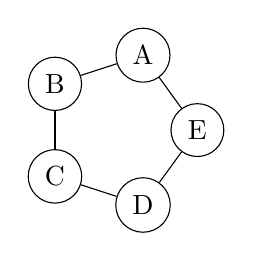
\begin{tikzpicture}
            % Define the positions of the nodes in a smaller pentagon
            \foreach \i/\name in {1/A, 2/B, 3/C, 4/D, 5/E} {
                \node[circle, draw, minimum size=0.4cm] (\name) at ({72*\i}:1cm) {\name};
            }
        
            % Connect the nodes to form a pentagon
            \foreach \i/\j in {A/B, B/C, C/D, D/E, E/A} {
                \draw (\i) -- (\j);
                }
        \end{tikzpicture}
    \end{center}

    DFS starting from $A$ follows:
    \[
    A \rightarrow B \rightarrow C \rightarrow E \rightarrow D
    \]
\end{exampletcb}

% Next section

\section{Breadth-First Search (BFS)}
\begin{algorithmtcb}
    {Breadth-First Search}{bfs}
    \begin{algorithmic}
        \State Given a graph $G = (V, E)$ and starting node $s$
        \State Initialize queue with $s$, mark $s$ as visited
        \While{queue is not empty}
            \State Dequeue node $v$ from queue
            \For{each unvisited neighbor $w$ of $v$}
                \State Mark $w$ as visited
                \State Enqueue $w$
            \EndFor
        \EndWhile
    \end{algorithmic}
\end{algorithmtcb}

\begin{exampletcb}
    {Breadth-First Search}{example_bfs}
    Consider a graph:
\begin{center}
    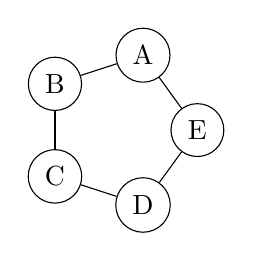
\begin{tikzpicture}
        % Define the positions of the nodes in a smaller pentagon
        \foreach \i/\name in {1/A, 2/B, 3/C, 4/D, 5/E} {
            \node[circle, draw, minimum size=0.4cm] (\name) at ({72*\i}:1cm) {\name};
        }
    
        % Connect the nodes to form a pentagon
        \foreach \i/\j in {A/B, B/C, C/D, D/E, E/A} {
            \draw (\i) -- (\j);
            }
    \end{tikzpicture}
\end{center}
    BFS starting from $A$ follows:
    \[
    A \rightarrow B \rightarrow D \rightarrow C \rightarrow E
    \]
\end{exampletcb}
